% !TEX root = ./../../main.tex
\subsection{Using the Maximum Likelihood Estimator to Find Parameters}
\label{sec:analysis:mle}

Another way of finding fit parameters for a model is the \quotedef{Maximum Likelihood Estimator} method. For this part, we will analyze simulated data from a radioactive decay, which will be generated within the code. Specifically, we will match a fit function (\autoref{eq:mle:decay_function}) to the lifetimes of decaying particles. This function takes the mean lifetime \( \tau \) as a parameter, so finding the fit function also returns this an estimate of this value.
\begin{gather}
    f(t \given \tau) = \frac{1}{\tau} e^{-t/\tau}
    \label{eq:mle:decay_function}
\end{gather}

The \define{likelihood} function \( L \) is defined as the probability of finding the measured data, given the parameters of a model.
For independent measurements this factorizes nicely:
\begin{equation}
    L(\vec{x} \given \vec{λ}) = \prod_{x_i \in \vec{x}} f(x_i \given \vec{λ}).
\end{equation}
The point is that the likelihood function treats the parameter as the independent variable.
This lets us estimate the parameter by maximizing the likelihood.
Equivalently, it is often easier to maximize the \define{log-likelihood} function.

\subsubsection{Applying the MLE Method to find a Fit Parameter with Uncertainty}

Using the MLE method, the goal is to find the fit parameters (in this case \( \tau \)) which maximize the likelihood that the data came from the distribution. This is a reasonable way of estimating the parameters of the distribution, as we are assuming that nothing extremely unlikely happened during measurement (as that would by definition be unlikely to happen). In this case, we can find the parameter \( \tau \) by solving analytically.

We start with the general log-likelihood function. Inserting the decay distribution function $f(t \given \tau)$ from \autoref{eq:mle:decay_function} and simplifying gives us a different expression for the log-likelihood.
\begin{align}
    \ln L(\vec{t} \given \tau) &= \sum \limits_{i = 1}^{n} \ln f(t_i \given \tau) \\
    &= \sum \limits_{i = 1}^{n} \ln \Big( \frac{1}{\tau} e^{\frac{-t_i}{\tau}} \Big) \\
    &= \sum \limits_{i = 1}^{n} \Big( - \ln (\tau) - \frac{t_i}{\tau} \Big) \\
    &= - n \ln (\tau) - \frac{1}{\tau} \sum \limits_{i = 1}^{n} t_i \\
\end{align}

It is much easier to take the derivative in this form. Because the logarithm is monotonic, the maximum of the likelihood will be at the same point as the maximum of the log-likelihood. This is at the inflection point of the function, where the first derivative is zero.
\begin{gather}
    \frac{\partial}{\partial \tau} \ln L(\vec{t} \given \tau) = -\frac{n}{\tau} + \frac{1}{\tau^2} \sum \limits_{i = 1}^{n} t_i \\
    \frac{n}{\tau} = \frac{1}{\tau^2} \sum \limits_{i = 1}^{n} t_i \\
    \tau = \frac{1}{n} \sum \limits_{i = 1}^{n} t_i := \hat{\tau}
    \label{eq:mle:tau_hat_mle}
\end{gather}

The calculated value \( \hat{\tau} \) is called the maximum likelihood estimate of \( \tau \). This is the fit parameter, which is why it gets a new symbol. We note that in this case the MLE is simply the average of the measurements. This is to be expected because the parameter \( \tau \) \emph{is} the mean lifetime.

To find the uncertainty of this estimate, we compute the second derivative and insert this into the known equation for $\sigma_\tau^2$.
\begin{align}
    \frac{\partial^2}{\partial \tau^2} \ln L(\vec{t} \given \tau) &= \frac{n}{\tau^2} - \frac{2}{\tau^3} \sum \limits_{i = 1}^{n} t_i \\
    &= \frac{n}{\tau^2} - \frac{2 n}{\tau^3} \cdot \frac{1}{n} \sum \limits_{i = 1}^{n} t_i \\
    &= \frac{n}{\tau^2} - \frac{2 n \hat{\tau}}{\tau^3}
\end{align}

Lastly we can evaluate the second derivative at $\tau = \hat{\tau}$ and use it in the known equation for $\sigma_\tau^2$.

\begin{align}
    \sigma_\tau^2 &= - \left(\frac{\partial^2 \ln L(\tau)}{\partial^2 \tau} \Big|_{\tau = \hat{\tau}} \right)^{-1} \\
    &= - \left(- \frac{n}{\hat{\tau}^2} \right)^{-1} \\
    \sigma_\tau &= \frac{\hat{\tau}}{\sqrt{n}}
    \label{eq:mle:uncertainty_of_tau_hat}
\end{align}

We arrive at \autoref{eq:mle:uncertainty_of_tau_hat}, which gives the uncertainty of \( \hat{\tau} \). Along with the equation for the MLE of \( \hat{\tau} \) itself (\autoref{eq:mle:tau_hat_mle}), we can calculate the parameters of the distribution which produced the data.

\subsubsection{Plotting the Log-Likelihood Function and its Approximation}

To understand the shapes of log-likelihood functions better, we generate some data from the distribution \autoref{eq:mle:decay_function}, using the true value of \( \tau = \num{2} \). The log-likelihood function is calculated and plotted for different values of the parameter \( \tau \) for datasets with \( n \in \{ 30, 300 \} \) data points (see \autoref{fig:mle:lllh}).

We will also plot the second order approximation of the log-likelihood function. With both functions on the same graph, we can examine how well the approximation holds. The resulting graphs will be explained in the discussion.
\begin{gather}
    \ln L(\tau) \approx \ln L_\mathrm{max} - \frac{(\tau - \hat{\tau})^2}{2 \sigma_\tau^2}
\end{gather}

\begin{figure}
    \centering
    \begin{subfigure}{.4\textwidth}
        \centering
        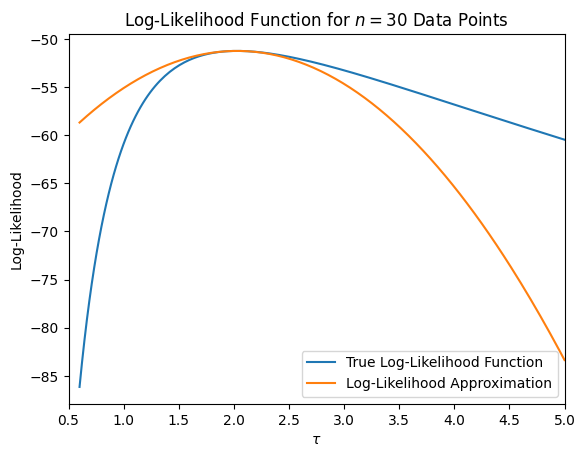
\includegraphics[width=.9\textwidth]{Graphs/MLE/lllh_for_30_data_points.png}
        \caption{\( n = 30 \)}
        \label{fig:mle:lllh_30_data_points}
    \end{subfigure}
    \begin{subfigure}{.4\textwidth}
        \centering
        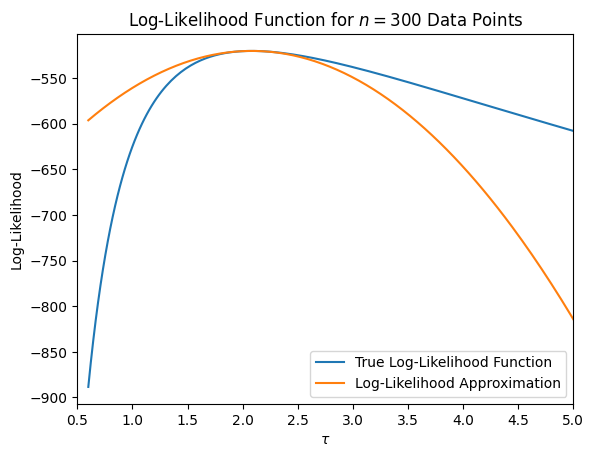
\includegraphics[width=.9\textwidth]{Graphs/MLE/lllh_for_300_data_points.png}
        \caption{\( n = 300 \)}
        \label{fig:mle:lllh_300_data_points}
    \end{subfigure}
    % \begin{subfigure}{.4\textwidth}
    %     \centering
    %     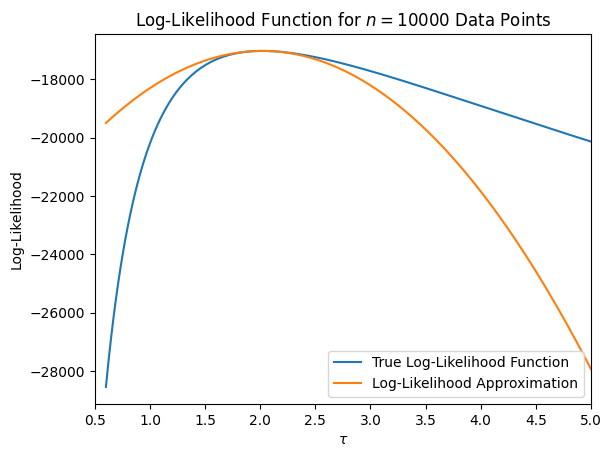
\includegraphics[width=.9\textwidth]{Graphs/MLE/lllh_for_10000_data_points.png}
    %     \caption{\( n = 10000 \)}
    %     \label{fig:mle:lllh_10000_data_points}
    % \end{subfigure}
    \caption{Exact and Approximated Log-Likelihood Functions for \( n \) Data Points.}
    \label{fig:mle:lllh}
\end{figure}

\subsubsection{Effectiveness of the MLE Method}

We will now examine how effective the MLE method really is at finding/predicting the correct \( \tau \).

In this case we define a prediction of \( \tau \) as \quotedef{successful} if the true value of $\tau$ is within a \qty{1}{\sigma} interval of our (MLE) prediction $\hat{\tau}$. We generate data many times and run the analysis each time, counting how many calculations of \( \hat{\tau} \) are near \num{2}, the true value of \( \tau \).

By generating many data sets with large numbers of samples, we approximate the long-term expected number of successful predictions of $\tau$. Following the frequentist interpretation of probability, the long-term ratio of successes to failures is by definition the probability of success.

From the total number of runs and the number of successes we can calculate the success ratio: For \num{1000} data sets of \num{500} samples, we get about \num{670} successful predictions, meaning a success rate of \qty{67}{\percent}.

% discuss how good 67 percent is?
% not that important, happy to ignore

\subsection{MLE Analysis on a Second Dataset}

We want to examine another generated dataset (see attached \verb|.csv| files). For this one, the probability density function for the distribution of an angle $\alpha$ is given by \autoref{eq:mle:pdf_02}.
\begin{gather}
    f(x\given a) = \frac{1 + a x}{2}, \quad x = \cos \alpha
    \label{eq:mle:pdf_02}
\end{gather}

The parameter $a$ is in the range $-1 \le a \le 1$.

For the generated dataset $\vec{x}$ with $n$ values, the log-likelihood of is therefore:

\begin{align}
    \ln L(\vec{x}\given a) &= \sum \limits_{i=1}^{n} \ln f(\vec{x}\given a) \\
    \ln L(\vec{x}\given a) &= \sum \limits_{i=1}^{n} \ln \frac{1 + a x_i}{2}
\end{align}

Using the same MLE method and numerical minimization tool \texttt{iminuit} with this new function, we obtain the maximum likelihood estimate $\hat{a} = \num{0.19 \pm 0.05}$.

To confirm this result, the log-likelihood function and the MLE parameter are plotted in \autoref{fig:mle:lllh_part_02}. Visually we can confirm that $\hat{a}$ maximizes the likelihood of obtaining the given dataset $\vec{x}$.

\begin{figure}
    \centering
    \begin{subfigure}{.4\textwidth}
        \centering
        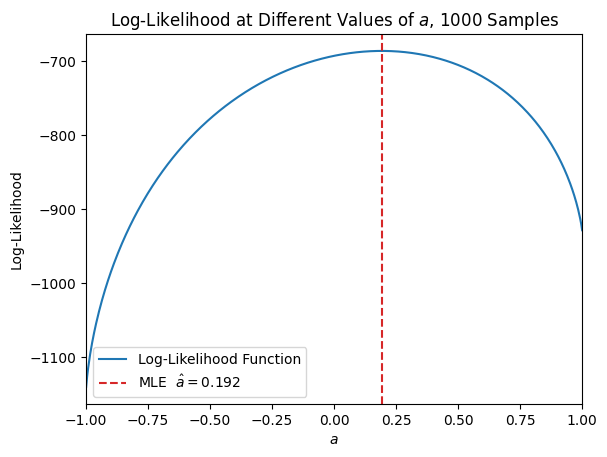
\includegraphics[width=0.9\textwidth]{Graphs/MLE/lllh_part_02.png}
        \caption{Log-Likelihood Function using Generated Data Set with \( n = 1000 \) Samples}
        \label{fig:mle:lllh_part_02}
    \end{subfigure}
    \begin{subfigure}{.4\textwidth}
        \centering
        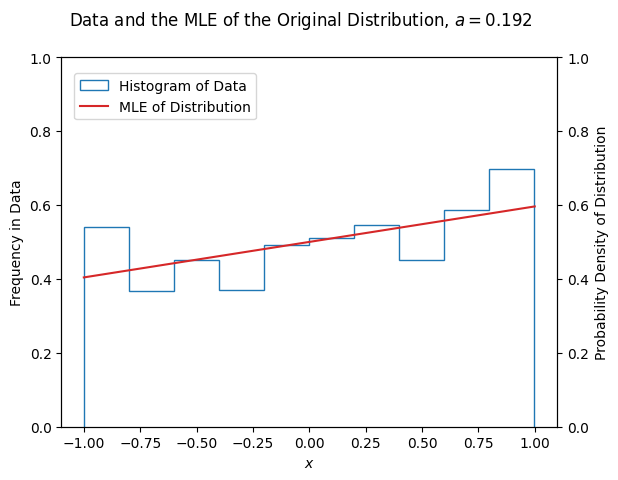
\includegraphics[width=0.9\textwidth]{Graphs/MLE/data_and_mle_part_02.png}
        \caption{Generated Data Alongside the Calculated Fit Function}
        \label{fig:mle:data_and_mle_part_02}
    \end{subfigure}
    \caption{MLE Method Applied to a Generated Dataset}
\end{figure}

\subsubsection{Plotting the Fit Function}

We plot the histogram of the data and the distribution function (using our determined fit parameter $\hat{a}$) on the same graph. We make sure to graph the histogram using density/relative frequency. This ensures that we have the same scaling for both elements in the graph, which visually shows that the shape of the histogram matches relatively well with the distribution. We can therefore see that the type of distribution is correct and that the estimate $\hat{a}$ for the parameter $a$ is generally accurate. The next section on errors will show this numerically.

\subsubsection{Determining Convergence of Upper and Lower Uncertainties}

We want to analyze the upper and lower errors of the MLE approach. These $\sigma_a^-$ and $\sigma_a^+$ are defined in \autoref{eq:mle:part_02_sigma_pm_definition}. We can rearrange this equation to define a new function $f$. The roots of this function give the desired solutions (the values of $\hat{a} \pm \sigma_a$).
\begin{align}
    \ln L_\mathrm{max} - \frac{1}{2} &= \ln L (\hat{a} \pm \sigma_a)
    \label{eq:mle:part_02_sigma_pm_definition} \\
    f(\hat{a} \pm \sigma_a) = 0 &= \ln L (\hat{a} \pm \sigma_a)  - \big( \ln L_\mathrm{max} - \frac{1}{2} \big)
\end{align}

Now we can use the standard \texttt{scipy.optimize.root\_scalar} function to find these roots and solve for the positive and negative deviations from \( \hat{a} \). The results for different data sets will be explained in the discussion.
\begin{gather}
    f(\hat{a} \pm \sigma_a) = 0 \\
    \Rightarrow a^+ = \hat{a} + \sigma_a^+ \\
    \Rightarrow a^- = \hat{a} - \sigma_a^- \\
    \sigma_a^+ = a^+ - \hat{a} \\
    \sigma_a^- = \hat{a} - a^-
\end{gather}